\documentclass{article}%
\usepackage[T1]{fontenc}%
\usepackage[utf8]{inputenc}%
\usepackage{lmodern}%
\usepackage{textcomp}%
\usepackage{lastpage}%
\usepackage{authblk}%
\usepackage{graphicx}%
%
\title{Autocrine production of interleukin{-}8 confers cisplatin and paclitaxel resistance in ovarian cancer cells}%
\author{Alexis Shepherd}%
\affil{School of Biosciences, University of Birmingham, Edgbaston, Birmingham B15 2TT, UK}%
\date{01{-}01{-}2014}%
%
\begin{document}%
\normalsize%
\maketitle%
\section{Abstract}%
\label{sec:Abstract}%
SAN DIEGO {-} Various corticosteroids and nonsteroidal anti{-}inflammatory drugs are associated with skeletal inflammation. Unfortunately, there are no therapies that are perfect for each individual, or which cause the disease as a whole. Treatment for this cause is difficult and the best option is current non{-}steroidal anti{-}inflammatory drugs (NSAIDs) which are used to prevent inflammation in order to alleviate pain.\newline%
Skeletal inflammation can lead to deformities, swelling and muscle disc issues. The condition leads to bone fractures, weak bones and various headaches, headaches have been linked to NODs, and hyperplasia. According to the Mayo Clinic, pain is one of the most common reasons for NODs. SAEs and nonsteroidal anti{-}inflammatory drugs (NSAIDs) are commonly used as pain relievers to prevent them from exacerbating, but there are other options.\newline%
Stress, grief, anxiety, lack of sleep, hormones and the alcohol factor are all potential NOD triggers, but researchers don't know why one makes the other more effective. A new study, published in the Journal of Bone and Mineral Research, reveals that by applying selective doses of selective DNA (SCDI) DNA in muscle tissue with collagen 3{-}hydroxylation systems, we may be able to increase the effect of opioid{-}containing drugs such as nonsteroidal anti{-}inflammatory drugs (NSAIDs) by up to 15 times.\newline%
After adjusting for the endogenous genetic variability and metabolic factors, the researchers found that this approach increases the beneficial effects of these nonsteroidal agents to approximately 20{-}25 times.\newline%
Learn more about SCDI DNA at SCDIForensics.com or related.

%
\subsection{Image Analysis}%
\label{subsec:ImageAnalysis}%


\begin{figure}[h!]%
\centering%
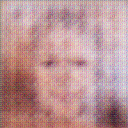
\includegraphics[width=150px]{500_fake_images/samples_5_324.png}%
\caption{A Man With A Beard Wearing A Tie}%
\end{figure}

%
\end{document}